\documentclass[a4paper,12pt]{article} 
\usepackage{mathrsfs}
\usepackage[utf8]{inputenc}
\usepackage[spanish]{babel}
\usepackage{amsmath}
\usepackage{amsfonts}
\usepackage{amssymb} 
\usepackage{graphicx} 
\usepackage{hyperref} 
\usepackage{wrapfig}
\usepackage{enumitem}
\usepackage{fancyhdr}
\usepackage{float}
\usepackage{eurosym}
\usepackage{color}
\usepackage{circuitikz}
\usepackage{titling}
\usepackage{hyperref}
\usepackage{media9}
\usepackage{lipsum}
\usepackage{tocbibind}
\usepackage{listings}
\usepackage{tabularx}
\usepackage{tcolorbox}
\usepackage{bookmark}
\usepackage{media9}
\usepackage[table]{xcolor}
\definecolor{lightblue}{RGB}{228, 244, 253}
\usepackage{listings}
\usepackage{color}

\definecolor{dkgreen}{rgb}{0,0.6,0}
\definecolor{gray}{rgb}{0.5,0.5,0.5}
\definecolor{mauve}{rgb}{0.58,0,0.82}

\lstset{frame=tb,
  language=Python,
  inputencoding=utf8,
  extendedchars=true,
  aboveskip=3mm,
  belowskip=3mm,
  showstringspaces=false,
  columns=flexible,
  basicstyle={\small\ttfamily},
  numbers=none,
  numberstyle=\tiny\color{gray},
  keywordstyle=\color{blue},
  commentstyle=\color{dkgreen},
  stringstyle=\color{mauve},
  breaklines=true,
  breakatwhitespace=true,
  tabsize=3,
  literate=%
    {á}{{\'a}}1
    {é}{{\'e}}1
    {í}{{\'i}}1
    {ó}{{\'o}}1
    {ú}{{\'u}}1
    {ñ}{{\~n}}1
    {č}{{\v{c}}}1
}
\usepackage[left=3cm,right=3cm,top=3cm,bottom=4cm]{geometry}
\sloppy

\pagestyle{fancy}
\providecommand{\abs}[1]{\lvert#1\rvert}
\providecommand{\norm}[1]{\lVert#1\rVert}

%%% Para las cabeceras
\newcommand{\hsp}{\hspace{20pt}}
\newcommand{\HRule}{\rule{\linewidth}{0.5mm}}
\headheight=50pt
%%% 
\newcommand{\vacio}{\textcolor{white}{ .}}

%%% Para que las ecuaciones se numeren
%%% con el número de sección y el de ecuación.
\renewcommand{\theequation}{\thesection.\arabic{equation}}


% Color azul para algunos 
% textos de la portada
\definecolor{azulportada}{rgb}{0.16, 0.32, 0.75}

%%%% Azul para textos de headings
\definecolor{azulinterior}{rgb}{0.0, 0.2, 0.6}

%%%%%%%%%%%%%%%%%%%%%%%%%%%%%%%%
%%%%%% Datos del proyecto %%%%%%
%%%%%%%%%%%%%%%%%%%%%%%%%%%%%%%%
%%%TÍTULO
%%% Escribirlo en minúsculas, el programa
%%% lo pondrá en mayúsculas en la portada.

\title{AirTrackPad}

%%%% AUTORES
\author{Lydia Ruiz Martínez \and Pablo Tuñón Laguna}

%%%%%%%%%%%%%%%%%%%%%
%%%%%%%%%%%%%%%%%%%%
\begin{document}

%%%%%%%%%%%%%%%%%%%%%%%%%%%%%%%
%%%%%%%%%%%%%%%%%%%%%%%%%%%%%%%
\begin{titlepage} %%%%% Aquí no hay que tocar nada.
	%%%% Las siguientes instrucciones generarán automáticamente
	%%%% la portada de tu proyecto.
	%%% Cambio de la estructura de esta página
\newgeometry{left=0.6cm,top=1.3cm,bottom=1.2cm}

\fbox{\parbox[c]{18.5cm}{
\begin{center}
\vspace{1.5cm}
{\fontfamily{ptm}\fontsize{24}{28.8}\selectfont{Universidad Pontificia Comillas}}\\
[2.5em]
{\fontfamily{ptm}\fontsize{24}{5}\selectfont{ETSI-ICAI}}\\
[3.5em]
{\fontfamily{ptm}\fontsize{28}{5}\selectfont{Research documentation}}\\
[3cm]
% {\fontfamily{ptm}\fontsize{24}{5}\selectfont{Visión por Ordenador I}}\\
% [2cm]

% Autor del trabajo de investigación
\textcolor{azulportada}
{\fontfamily{ptm}\fontsize{45}{5}\selectfont{\textsc{\thetitle}}}\\
[3cm]
% Título del trabajo
\textcolor{azulportada}
{\fontfamily{ptm}\fontsize{16}{5}\selectfont{\theauthor}}\\
%{\Huge\textbf{\thetitle}}\\
[1.2cm]

\includegraphics[width=10cm]{contents/Logo ICAI.png}
\\[1.8cm]

{\fontfamily{ptm}\fontsize{16}{5}\selectfont{December 2024}}\\
[4cm]
\end{center}
}}
\end{titlepage}
 
 \restoregeometry
 %%%% Volvemos a la estructura de la página normal

%%%%%%%%%%%%%%%%%%%%%%%%%%%%%%

{%\Large

%%%Encabezamiento y pie de página
%%% También se genera automáticamente
%%% Mejor no tocarlo mucho.
\renewcommand{\headrulewidth}{0.5pt}
\fancyhead[R]{
\textcolor{azulportada}{\fontfamily{ptm}\fontsize{10}{3}\selectfont{Proyecto Final de Visión por Ordenador I}}\\
{\fontfamily{ptm}\fontsize{10}{3}\selectfont{\theauthor}}}
\fancyhead[L]{
  \textcolor{azulinterior}{\fontfamily{ptm}\fontsize{12}{4}\selectfont{\textbf{\thetitle}}}\\
}


\pagestyle{fancy}
\renewcommand{\footrulewidth}{0.5pt}
\fancyfoot[L]{\footnotesize Universidad Pontificia Comillas (ICAI) --- curso 2024-2025}
\fancyfoot[C]{\vacio}
\fancyfoot[R]{\footnotesize Página \thepage}

%%%%%%%%%%%%%%%%%%%%

\newpage

\renewcommand{\contentsname}{Index of contents}
\addtocontents{toc}{\protect\setcounter{tocdepth}{-1}} % Quita el índice de la tabla de contenidos
\tableofcontents
\addtocontents{toc}{\protect\setcounter{tocdepth}{3}}

\newpage

\section{Introduction}

\vspace{0.5cm}

Human interaction with computers has evolved significantly, seeking more intuitive and polyvalent interfaces.
AirTrackPad is part of this trend, allowing devices to be controlled through hand gestures detected in the air, without the need for additional hardware such
as a Kinect or a Leap Motion. It has been developed to be used either on a capable computer or a Raspberry Pi, making it a versatile tool for different applications.
At the end of this document, there is also a part that explains how to modify and re-train the model with different gestures, making it more adaptable to different needs.

\vspace{0.5cm}

\section{Methodology}

The project has been structured in 7 directories, 2 main files and 1 utils file that helps coordinating some functions between the different modules. That structure
can be seen in the following list:

\begin{itemize}
  \item \textbf{3d files}: two specific accessories designed and 3D printed to improve the user experience while using an external camera.
  \item \textbf{actions\_handler}: responsible for managing the actions derived from the classified gestures.
  \item \textbf{camera\_calibration}: the environment for the camera calibration process.
  \item \textbf{hand\_tracking}: implements landmark detection with \texttt{Mediapipe} with the verification of Sobel.
  \item \textbf{movement\_classifier}: contains models and scripts for gesture classification through machine learning techniques.
  \item \textbf{movement\_follower}: is the responsible of continuing the movement of the landmarks between frames.
  \item \textbf{AirTrackPad.py\&AirTrackPadLinux}: main scripts that integrate and coordinates all modules of the system to create the final product.
  \item \textbf{utils.py}: auxiliary functions that some modules repeat its use.
\end{itemize}


\subsection{Camera Calibration}

The camera calibration process is essential to ensure the accuracy of the hand tracking system. It is carried out by capturing images of a chessboard 
pattern from different angles and distances, allowing the estimation of the intrinsic and extrinsic parameters of the camera. The calibration module 
provides a graphical interface to facilitate the process, generating the necessary files for the subsequent configuration of the tracking system.
The cameras used for this project are a Raspberry Pi Camera Module 3 and the webcam of a laptop. It is important to note that the calibration process
is independent for each camera. The intrinsic parameters of the external camera are:

\begin{equation}
K = \begin{pmatrix}
346.97 & 0.0 & 226.29 \\
0.0 & 347.78 & 129.31 \\
0.0 & 0.0 & 1.0
\end{pmatrix}
\end{equation}

\subsection{Hand Detection and Tracking}


At the beggining it was used a Canny filter over a MOG2 mask to detect the hand, however it was discarded due to the low performance of the system and due to the
high computational cost. The final solution was to use the \texttt{Mediapipe} library, which provides a robust identification of 21 key points (\textit{landmarks}) in the hand:

\begin{figure}[H]
  \centering
  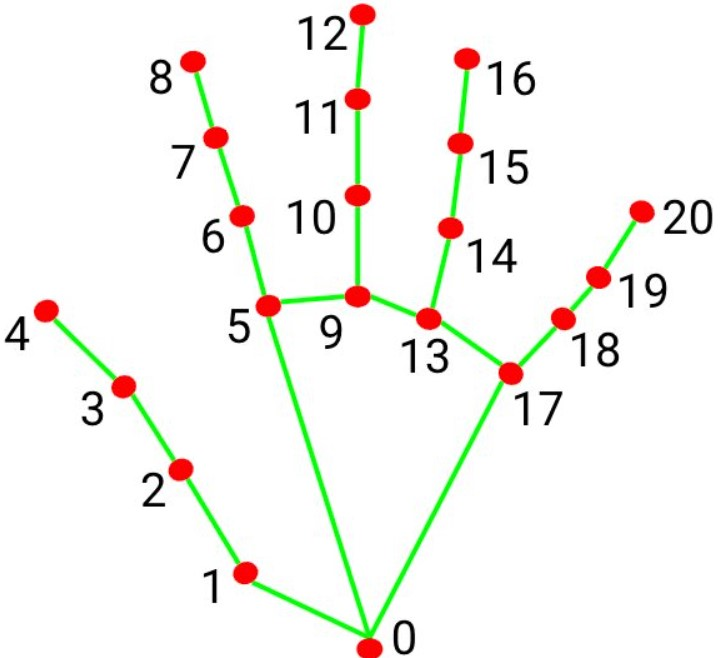
\includegraphics[width=0.35\textwidth]{contents/mediapipe.jpg}
  \caption{Hand landmarks detected by Mediapipe, ResearchGate}
  \label{fig:mediapipe}
\end{figure}

The landmarks detection of Mediapipe where complemented with a sobel filter over the ROI of the hand. This allowed to extract an accuracy of the model, changing the detection
of the landmarks when the landmarks were not detected correctly.

\subsection{Gesture completion}

As it has been mentioned, thet Mediapipe landmarks are considerabely accurate, however for the times where the Sobel filter detects that the performance is not optimal,
or in case the do disappear due to a phisical problem (like a hand occlusion), the system continues the movement of the previous landmarks using the Lucas-Kanade optical 
flow algorithm. It is applied to the ROI of the detected points, which means 21 different optical flows. This may sound as a highly computacional algorithm, however Sobel
and Lucas-Kanade have an option for devices with less computational power that reduce the padding of the ROIs and the number of iterations of the algorithm.

\subsection{Gesture Classification}

The classification of gestures was originally carried by a logistic regression model, however it wasn't very accurate. For this reason, a neural network was 
developed with a hidden layer of 10 neurons and ReLU activation function for the classification of gestures. The Raspberry Pi is a device that needed a lightweight 
architecture therefore after some tests, 10 neurons was identified as a model that allowed real time use of the device with an acceptable degree of classification success.

\subsection{Action Handling}

Classified the actions, the system needed to convert them into actions that the computer could understand. To tackle this problem, the library \texttt{pyautogui} was used that 
allowed to define actions such as scrolling, clicking or moving the cursor.

\vspace{0.5cm}

\section{Results}

A video has been uploaded to the contents directory that shows the system working. The AirTrackPad is capable of working in real time, with a frame rate of 30 fps without never 
loosing the hand and with a classification accuracy of around 90\%. 

\vspace{0.5cm}

\section{Future developments}

Although the system is already functional and identifies correctly many gestures, it doesn't detect at the perfection the 10 movements. Scrolling and 2 hand inputs are the 
gestures that have a lower accuracy. However this might be solved through a more extensive training. Another improvement that could be done is to add a new layer to the neural
network, which would allow to increase the accuracy of the model. Some tests where performed on this direction and although at the beggining the raspberry wasn't capable 
of running the model fluently, reducing the resolution of the camera gave some promising results. Finally the system could be improved by adding a user interface 
that allows more interaction and adaptability to the user.

\section{Trainment of the model}

As it has been mentioned, the model can be retrained with different gestures and more accurate datasets, to perform this, some modifications should be performed on 
the \texttt{movement\_classifier} directory, more specifically on the \texttt{train\_model.py} file. The user should modify the gestures and number of movements, 
it should also modify the line 109 of the \textit{ClassifierTrainer.py} to 14 x the number of gestures to use (number of features). Finally it should modify the 
number of features and gestures on the \textit{AirTrackPad.py} file.

\vspace{0.5cm}

The training process is very intuitive as there is a graphical interface that informs the user of the movement that is being trained as well as the number of pictures for
the identification. It is important that the user tries to make as many movements as possible to ensure the accuracy of the model. Another interesting feature of the 
training process is that the training process is not realized with a set of images and points but with a set of movements with context that allows the model to learn 
the movement in different situations.

\end{document}



